\markdownRendererHeadingOne{Thesis Phase I : Recap}\markdownRendererInterblockSeparator
{}\vspace*{2.7cm}\markdownRendererInterblockSeparator
{}{\huge{\textbf{Thesis Phase I : Recap}}}\markdownRendererInterblockSeparator
{}\end{frame}\markdownRendererInterblockSeparator
{}\begin{frame}{\huge{{\textbf{Recap}}}}\markdownRendererInterblockSeparator
{}\begin{columns} \begin{column}{0.6\textwidth} \vspace{-13mm} \uncover<1->{ \begin{itemize} \item The missing baryon problem \item BLAs : Way to probe WHIM \item Absorber towards PG 0003+158 \item BLA survey \end{itemize} } \end{column} \begin{column}{0.4\textwidth} \uncover<4->{\begin{figure}[!htbp] \centering 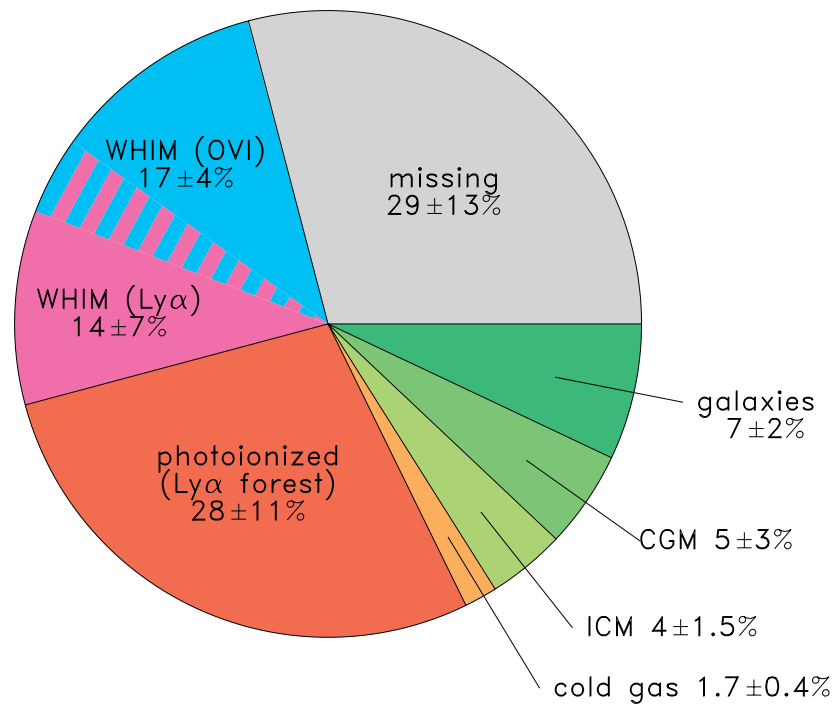
\includegraphics[width=5cm]{Figures/Mid-term/Baryon_distribution.png} \vspace*{-1mm} \caption{Baryon budget at $z \sim 0$. \\ Shull et al. (2012)} \label{} \end{figure}} \end{column} \end{columns}\markdownRendererInterblockSeparator
{}\begin{tikzpicture}[remember picture, overlay,use page relative coordinates]\markdownRendererInterblockSeparator
{}\uncover<2->{\node at (0.25,0.20) {Ref. : Fukugita et al. (1998)}} \uncover<4->{\node at (0.263,0.15) {Shull et al. (2012)}}\markdownRendererInterblockSeparator
{}\end{tikzpicture}\markdownRendererInterblockSeparator
{}\end{frame}\markdownRendererInterblockSeparator
{}\begin{frame}{\huge{{\textbf{Where are the Missing Baryons ?}}}}\markdownRendererInterblockSeparator
{}\uncover<1->{ \begin{itemize} \uncover<2->{\item Residing in sparse $(10^{-6}-10^{-4} \ cm^{-3})$ and hot ($10^{5}-10^{7}$ K) gas : WHIM} \uncover<3->{\item Low density - Undetectable emission signature} \uncover<4->{\item High temperature - Collisionally ionised} \end{itemize} }\markdownRendererInterblockSeparator
{}\begin{tikzpicture}[remember picture, overlay,use page relative coordinates]\markdownRendererInterblockSeparator
{}\uncover<2->{\node at (0.25,0.20) {Ref. : Cen and Ostriker (1999, 2006)}}\markdownRendererInterblockSeparator
{}\end{tikzpicture}\markdownRendererInterblockSeparator
{}\end{frame}\markdownRendererInterblockSeparator
{}\begin{frame}{\huge{{\textbf{How to detect WHIM ?}}}}\markdownRendererInterblockSeparator
{}\begin{columns} \begin{column}{0.35\textwidth} \vspace{-13mm} \uncover<1->{ \begin{itemize} \uncover<2->{\item Quasars as backlight} \begin{itemize} \uncover<4->{\item[-] \ion{O}{vi-viii}, \ \ion{Ne}{ix-x}, \ \ion{N}{vii}, etc.} \uncover<5->{\item[-] \textbf{BLAs}} \end{itemize} \end{itemize} } \end{column} \begin{column}{0.65\textwidth} \uncover<3->{ \begin{figure}[!htbp] \centering \includegraphics[width=9cm]{Figures/Mid-term/spec slice.png} \vspace*{-1mm} \caption{Slice of spectrum of quasar HE0153-4520 ($z_{em}=0.4510$). \ Danforth et al. (2016)} \end{figure}} \end{column} \end{columns}\markdownRendererInterblockSeparator
{}\begin{tikzpicture}[remember picture, overlay,use page relative coordinates]\markdownRendererInterblockSeparator
{}\uncover<4->{\node at (0.20,0.17) {Ref. : Tepper-García et al. (2013)} \node at (0.20,0.12) {Savage et al. (2014)}}\markdownRendererInterblockSeparator
{}\end{tikzpicture}\markdownRendererInterblockSeparator
{}\end{frame}\markdownRendererInterblockSeparator
{}\begin{frame}[noframenumbering]{\huge{{\textbf{How to detect WHIM ?}}}}\markdownRendererInterblockSeparator
{}\begin{columns} \begin{column}{0.35\textwidth} \vspace{-13mm} \begin{itemize} \item Quasars as backlight \begin{itemize} \item[-] \ion{O}{vi-viii}, \ \ion{Ne}{ix-x}, \ \ion{N}{vii}, etc. \item[-] \textbf{BLAs} \end{itemize} \end{itemize} \end{column} \begin{column}{0.65\textwidth} \uncover<1->{ \begin{figure}[!htbp] \centering 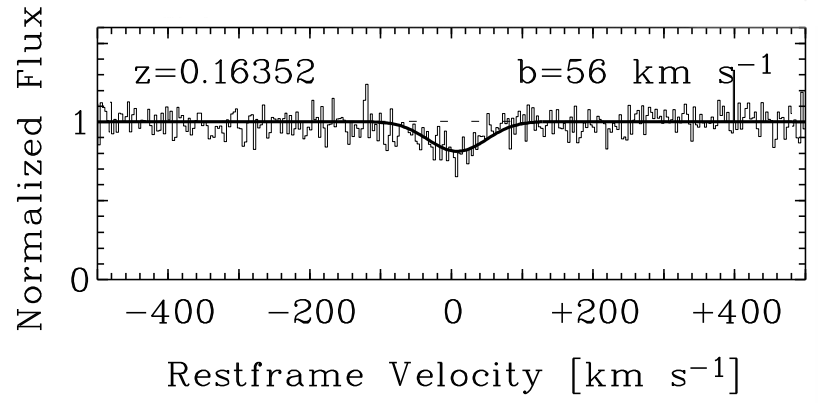
\includegraphics[width=9cm]{Figures/Mid-term/BLA-individual.png} \vspace*{-1mm} \caption{A BLA towards the LOS of quasar H 1821+643 $(z_{em} = 0.297)$ \\ Philipp Richter (2005)} \end{figure}} \end{column} \end{columns}\markdownRendererInterblockSeparator
{}\begin{tikzpicture}[remember picture, overlay,use page relative coordinates]\markdownRendererInterblockSeparator
{}\uncover<1->{\node at (0.20,0.17) {Ref. : Tepper-García et al. (2013)} \node at (0.20,0.12) {Savage et al. (2014)}}\markdownRendererInterblockSeparator
{}\end{tikzpicture}\markdownRendererInterblockSeparator
{}\end{frame}\markdownRendererInterblockSeparator
{}\begin{frame}[noframenumbering]{\huge{{\textbf{How to detect WHIM ?}}}}\markdownRendererInterblockSeparator
{}\begin{columns} \begin{column}{0.35\textwidth} \vspace{-13mm} \begin{itemize} \item Quasars as backlight \begin{itemize} \item[-] \ion{O}{vi-viii}, \ \ion{Ne}{ix-x}, \ \ion{N}{vii}, etc. \item[-] \textbf{BLAs} \end{itemize} \end{itemize} \end{column} \begin{column}{0.65\textwidth} \uncover<1->{ \begin{figure}[!htbp] \centering 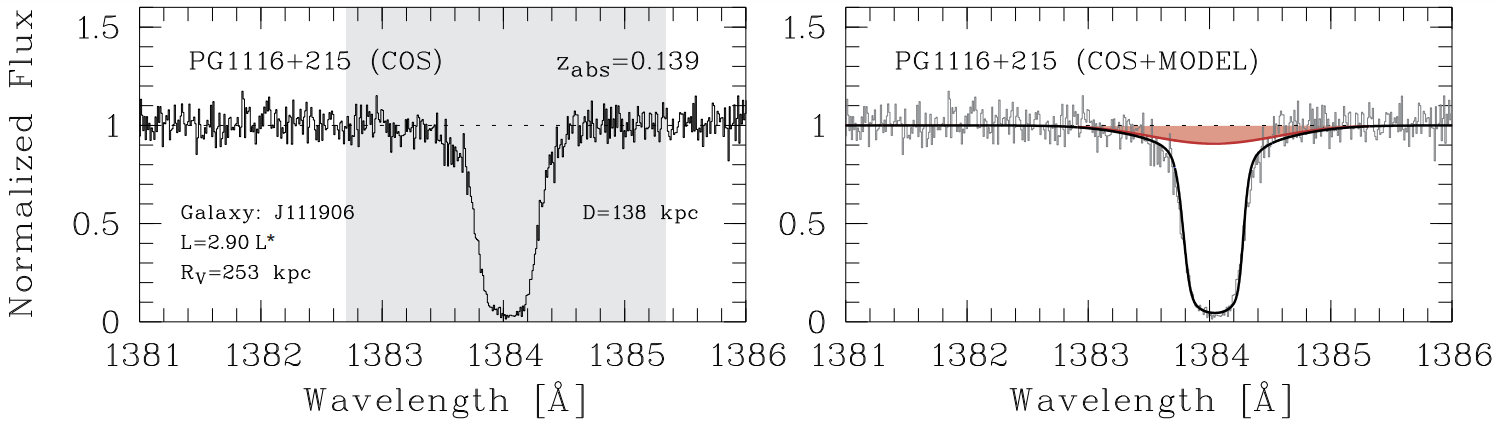
\includegraphics[width=9cm]{Figures/Mid-term/BLA.png} \vspace*{-1mm} \caption{A BLA blended with other Ly$\alpha$ absorption lines towards the LOS of quasar PG1116+215 $(z_{em} = 0.176)$. Philipp Richter (2020)} \end{figure}} \end{column} \end{columns}\markdownRendererInterblockSeparator
{}\begin{tikzpicture}[remember picture, overlay,use page relative coordinates]\markdownRendererInterblockSeparator
{}\uncover<1->{\node at (0.20,0.17) {Ref. : Tepper-García et al. (2013)} \node at (0.20,0.12) {Savage et al. (2014)}}\markdownRendererInterblockSeparator
{}\end{tikzpicture}\markdownRendererInterblockSeparator
{}\end{frame}\markdownRendererInterblockSeparator
{}\markdownRendererHeadingOne{Project Roadmap}\markdownRendererInterblockSeparator
{}\vspace*{2.7cm}\markdownRendererInterblockSeparator
{}{\huge{\textbf{Project Roadmap}}}\markdownRendererInterblockSeparator
{}\end{frame}\markdownRendererInterblockSeparator
{}\begin{frame}{\huge{\textbf{Roadmap}}}\markdownRendererInterblockSeparator
{}\uncover<1->{ \begin{itemize} \uncover<2->{\item \textbf{Phase 1}} \begin{itemize} \uncover<3->{\item[-] Detailed study of one absorber system} \uncover<4->{\item[-] Absorber along LOS of PG0003+158} \end{itemize} \vspace*{5mm} \uncover<2->{\item \textbf{Phase 2}} \begin{itemize} \uncover<5->{\item[-] Hunt for BLAs : An Exhaustive Survey} \uncover<6->{\item[-] Contribution of BLAs to $\Omega_b$} \end{itemize} \end{itemize} }\markdownRendererInterblockSeparator
{}\end{frame}\markdownRendererInterblockSeparator
{}\markdownRendererHeadingOne{Data}\markdownRendererInterblockSeparator
{}\vspace*{2.7cm}\markdownRendererInterblockSeparator
{}{\huge{\textbf{Data}}}\markdownRendererInterblockSeparator
{}\end{frame}\markdownRendererInterblockSeparator
{}\begin{frame}{\huge{{\textbf{\textit{HST}/COS Data}}}}\markdownRendererInterblockSeparator
{}\uncover<1->{\begin{itemize} \uncover<2->{\item 82 UV-bright AGNs chosen by Danforth et al. (2016) \uncover<3->{\item $z_{AGN} < 0.85$}} \uncover<4->{\item High S/N $\gtrsim$ 15} \uncover<5->{\item FUV channel : G130M and G160M gratings \uncover<6->{\item Coverage : 1130-1790 \AA}} \uncover<7->{\item $\text{R} \sim 17,000 \ \approx$ 17 km $\text{s}^{-1}$} \end{itemize}}\markdownRendererInterblockSeparator
{}\end{frame}\markdownRendererInterblockSeparator
{}\begin{frame}{\huge{{\textbf{Danforth et al. (2016) Datasets}}}}\markdownRendererInterblockSeparator
{}\markdownRendererUlBegin
\markdownRendererUlItem Reduced spectra\markdownRendererUlItemEnd 
\markdownRendererUlItem Identified lines\markdownRendererUlItemEnd 
\markdownRendererUlEnd \markdownRendererInterblockSeparator
{}\end{frame}\markdownRendererInterblockSeparator
{}\markdownRendererHeadingOne{Phase I}\markdownRendererInterblockSeparator
{}\vspace*{2.7cm}\markdownRendererInterblockSeparator
{}{\huge{\textbf{Phase I}}}\markdownRendererInterblockSeparator
{}\end{frame}\markdownRendererInterblockSeparator
{}\begin{frame}{\huge{{\textbf{Studying an Absorber System}}}}\markdownRendererInterblockSeparator
{}\uncover<1-> { \begin{itemize} \uncover<2->{ \item \textbf{I \ \ \ \ } \uncover<3->{: \hspace{1mm} Voigt profile fitting - VPFIT} \item \textbf{II \ \ \hspace{1pt}} \uncover<4->{: \hspace{1mm} Ionization modelling - CLOUDY} \item \textbf{III \ } \uncover<5->{: \hspace{1mm} Analyzing galaxy neighbourhood} } \end{itemize} }\markdownRendererInterblockSeparator
{}\end{frame}\markdownRendererInterblockSeparator
{}% \begin{frame}{\textbf{VPFIT}}\markdownRendererInterblockSeparator
{}% \begin{figure}[!htbp] % \hspace{-6cm} % \fbox{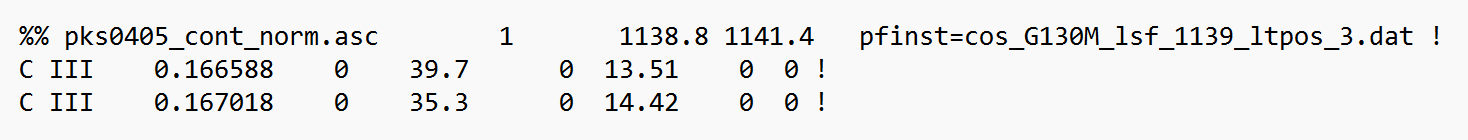
\includegraphics[width=10cm]{Figures/Mid-term/VPFIT_ip.png}} % \vspace*{-1mm} % \hspace{-6cm} % \caption{An example VPFIT input file} % \end{figure}\markdownRendererInterblockSeparator
{}% \begin{figure}[!htbp] % \centering % \fbox{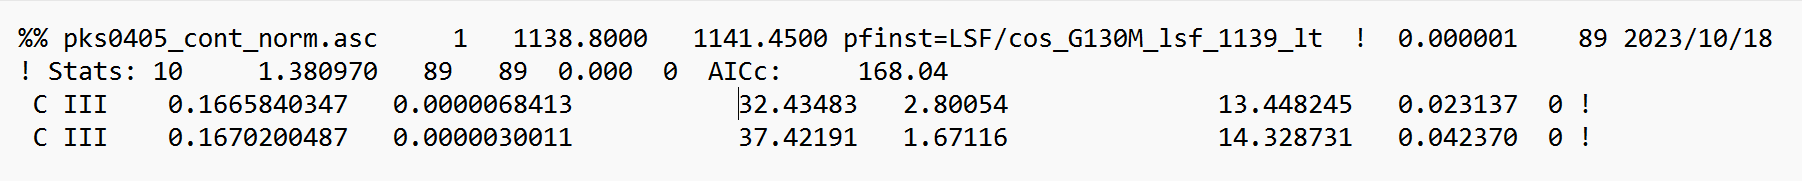
\includegraphics[width=12cm]{Figures/Mid-term/VPFIT_op.png}} % \vspace*{-1mm} % \caption{An example VPFIT output file} % \end{figure}\markdownRendererInterblockSeparator
{}% \end{frame}\markdownRendererInterblockSeparator
{}% \begin{frame}{\textbf{}}\markdownRendererInterblockSeparator
{}% \vspace*{-6mm}\markdownRendererInterblockSeparator
{}% \begin{figure}[!htbp] % \centering % 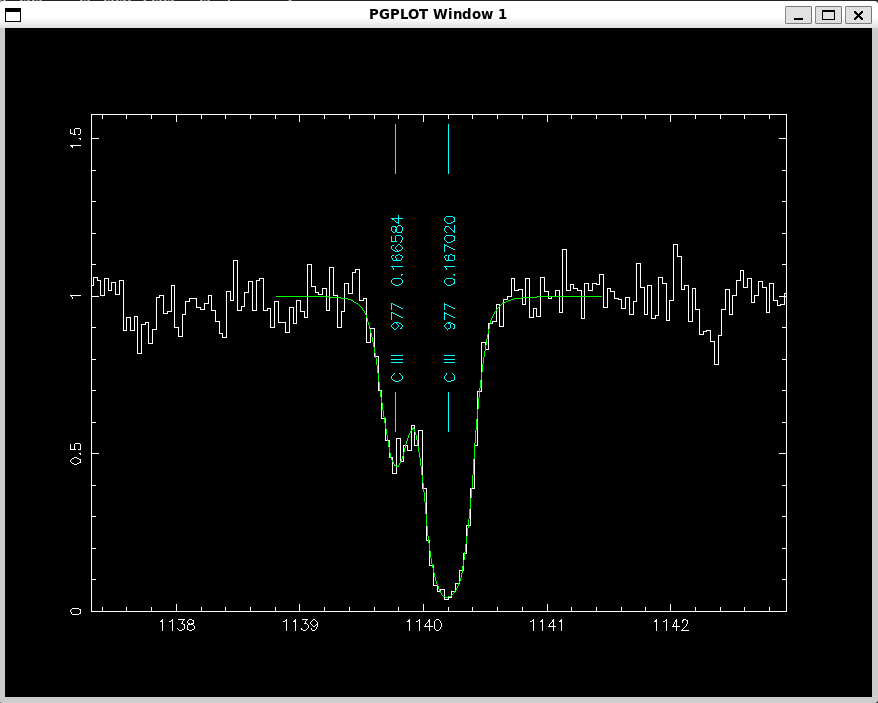
\includegraphics[width=7cm]{Figures/Mid-term/VPFIT_fit.png} % \vspace*{-1mm} % \caption{An example 2 component fit with VPFIT} % \end{figure}\markdownRendererInterblockSeparator
{}% \end{frame}\markdownRendererInterblockSeparator
{}% \begin{frame}{\textbf{CLOUDY}}\markdownRendererInterblockSeparator
{}% \uncover<1->{\begin{itemize} % \uncover<2->{\item Predicts thermal, ionization, and chemical structure of cloud} % \uncover<3->{\item Photoionization and Collisional ionization} % \uncover<4->{\item Models clouds as homogeneous plane parallel slabs} % \uncover<5->{\item Inputs : density, metallicity, {\color{red} temperature}, N(\ion{H}{i}), etc.} % \uncover<6->{\item Outputs : column densities, ionization fractions, {\color{red} temperature}, etc.} % \end{itemize}}\markdownRendererInterblockSeparator
{}% \end{frame}\markdownRendererInterblockSeparator
{}% \begin{frame}[noframenumbering]{\textbf{CLOUDY}}\markdownRendererInterblockSeparator
{}% \begin{figure}[!htbp] % \centering % 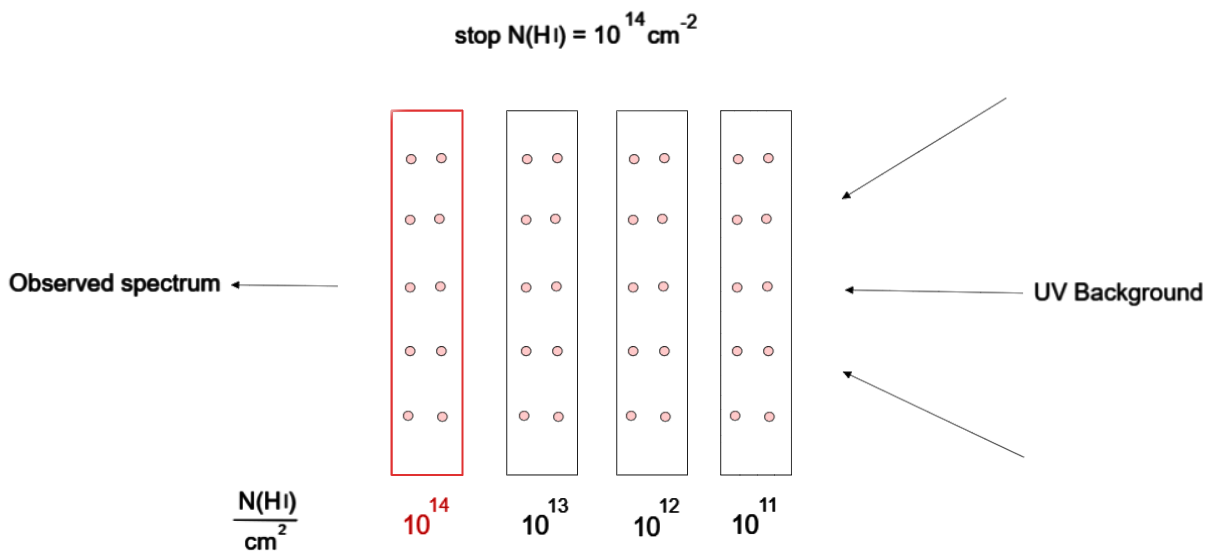
\includegraphics[width=12cm]{Figures/Mid-term/cloudy-3.png} % \vspace*{-1mm} % \caption{Schematic diagram of CLOUDY simulations.} % \end{figure}\markdownRendererInterblockSeparator
{}% \end{frame}\markdownRendererInterblockSeparator
{}\markdownRendererHeadingOne{Absorber system towards PG0003+158}\markdownRendererInterblockSeparator
{}\vspace*{2.7cm}\markdownRendererInterblockSeparator
{}{\huge{\textbf{Absorber system towards PG0003+158}}}\markdownRendererInterblockSeparator
{}\end{frame}\markdownRendererInterblockSeparator
{}\begin{frame}{\huge{{\textbf{Absorber system}}}}\markdownRendererInterblockSeparator
{}\markdownRendererUlBegin
\markdownRendererUlItem Quasar at $z_{em}=0.45089$\markdownRendererUlItemEnd 
\markdownRendererUlItem $z_{abs} \sim$ 0.347\markdownRendererUlItemEnd 
\markdownRendererUlItem 3 component system\markdownRendererUlItemEnd 
\markdownRendererUlEnd \markdownRendererInterblockSeparator
{}\begin{figure}[!htbp] \centering 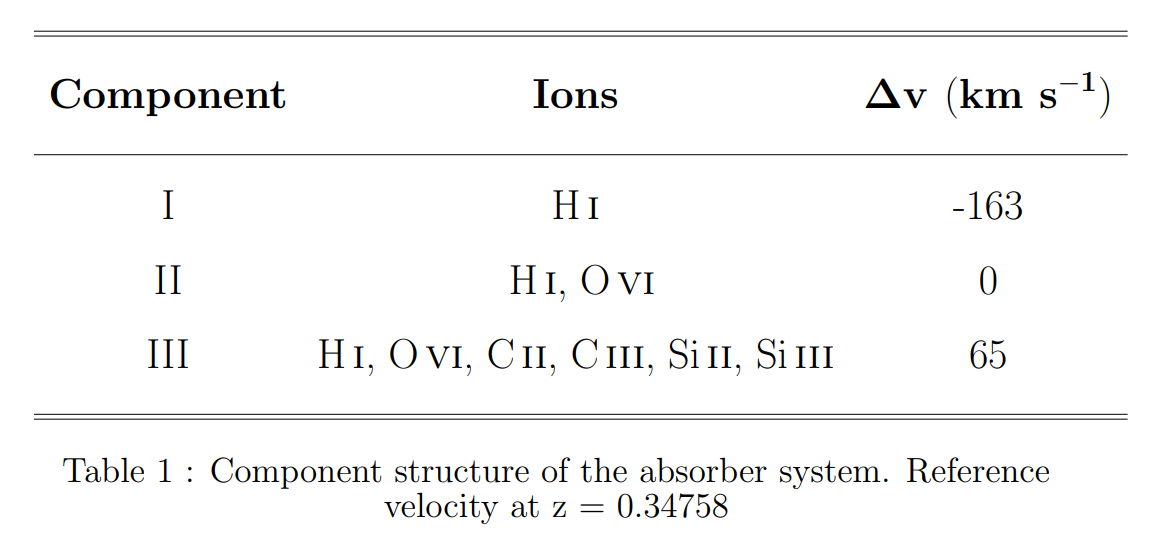
\includegraphics[width=7cm]{Figures/Mid-term/Component_structure2.png} \end{figure}\markdownRendererInterblockSeparator
{}\end{frame}\markdownRendererInterblockSeparator
{}\begin{frame}{\huge{{\textbf{Voigt profile fitting}}}}\markdownRendererInterblockSeparator
{}\end{frame}\markdownRendererInterblockSeparator
{}% ### \huge{{\textbf{Voigt profile fitting results}}} % \begin{frame}<presentation:0>[plain,noframenumbering]\markdownRendererInterblockSeparator
{}% % \begin{figure}[!htbp] % % \centering % % 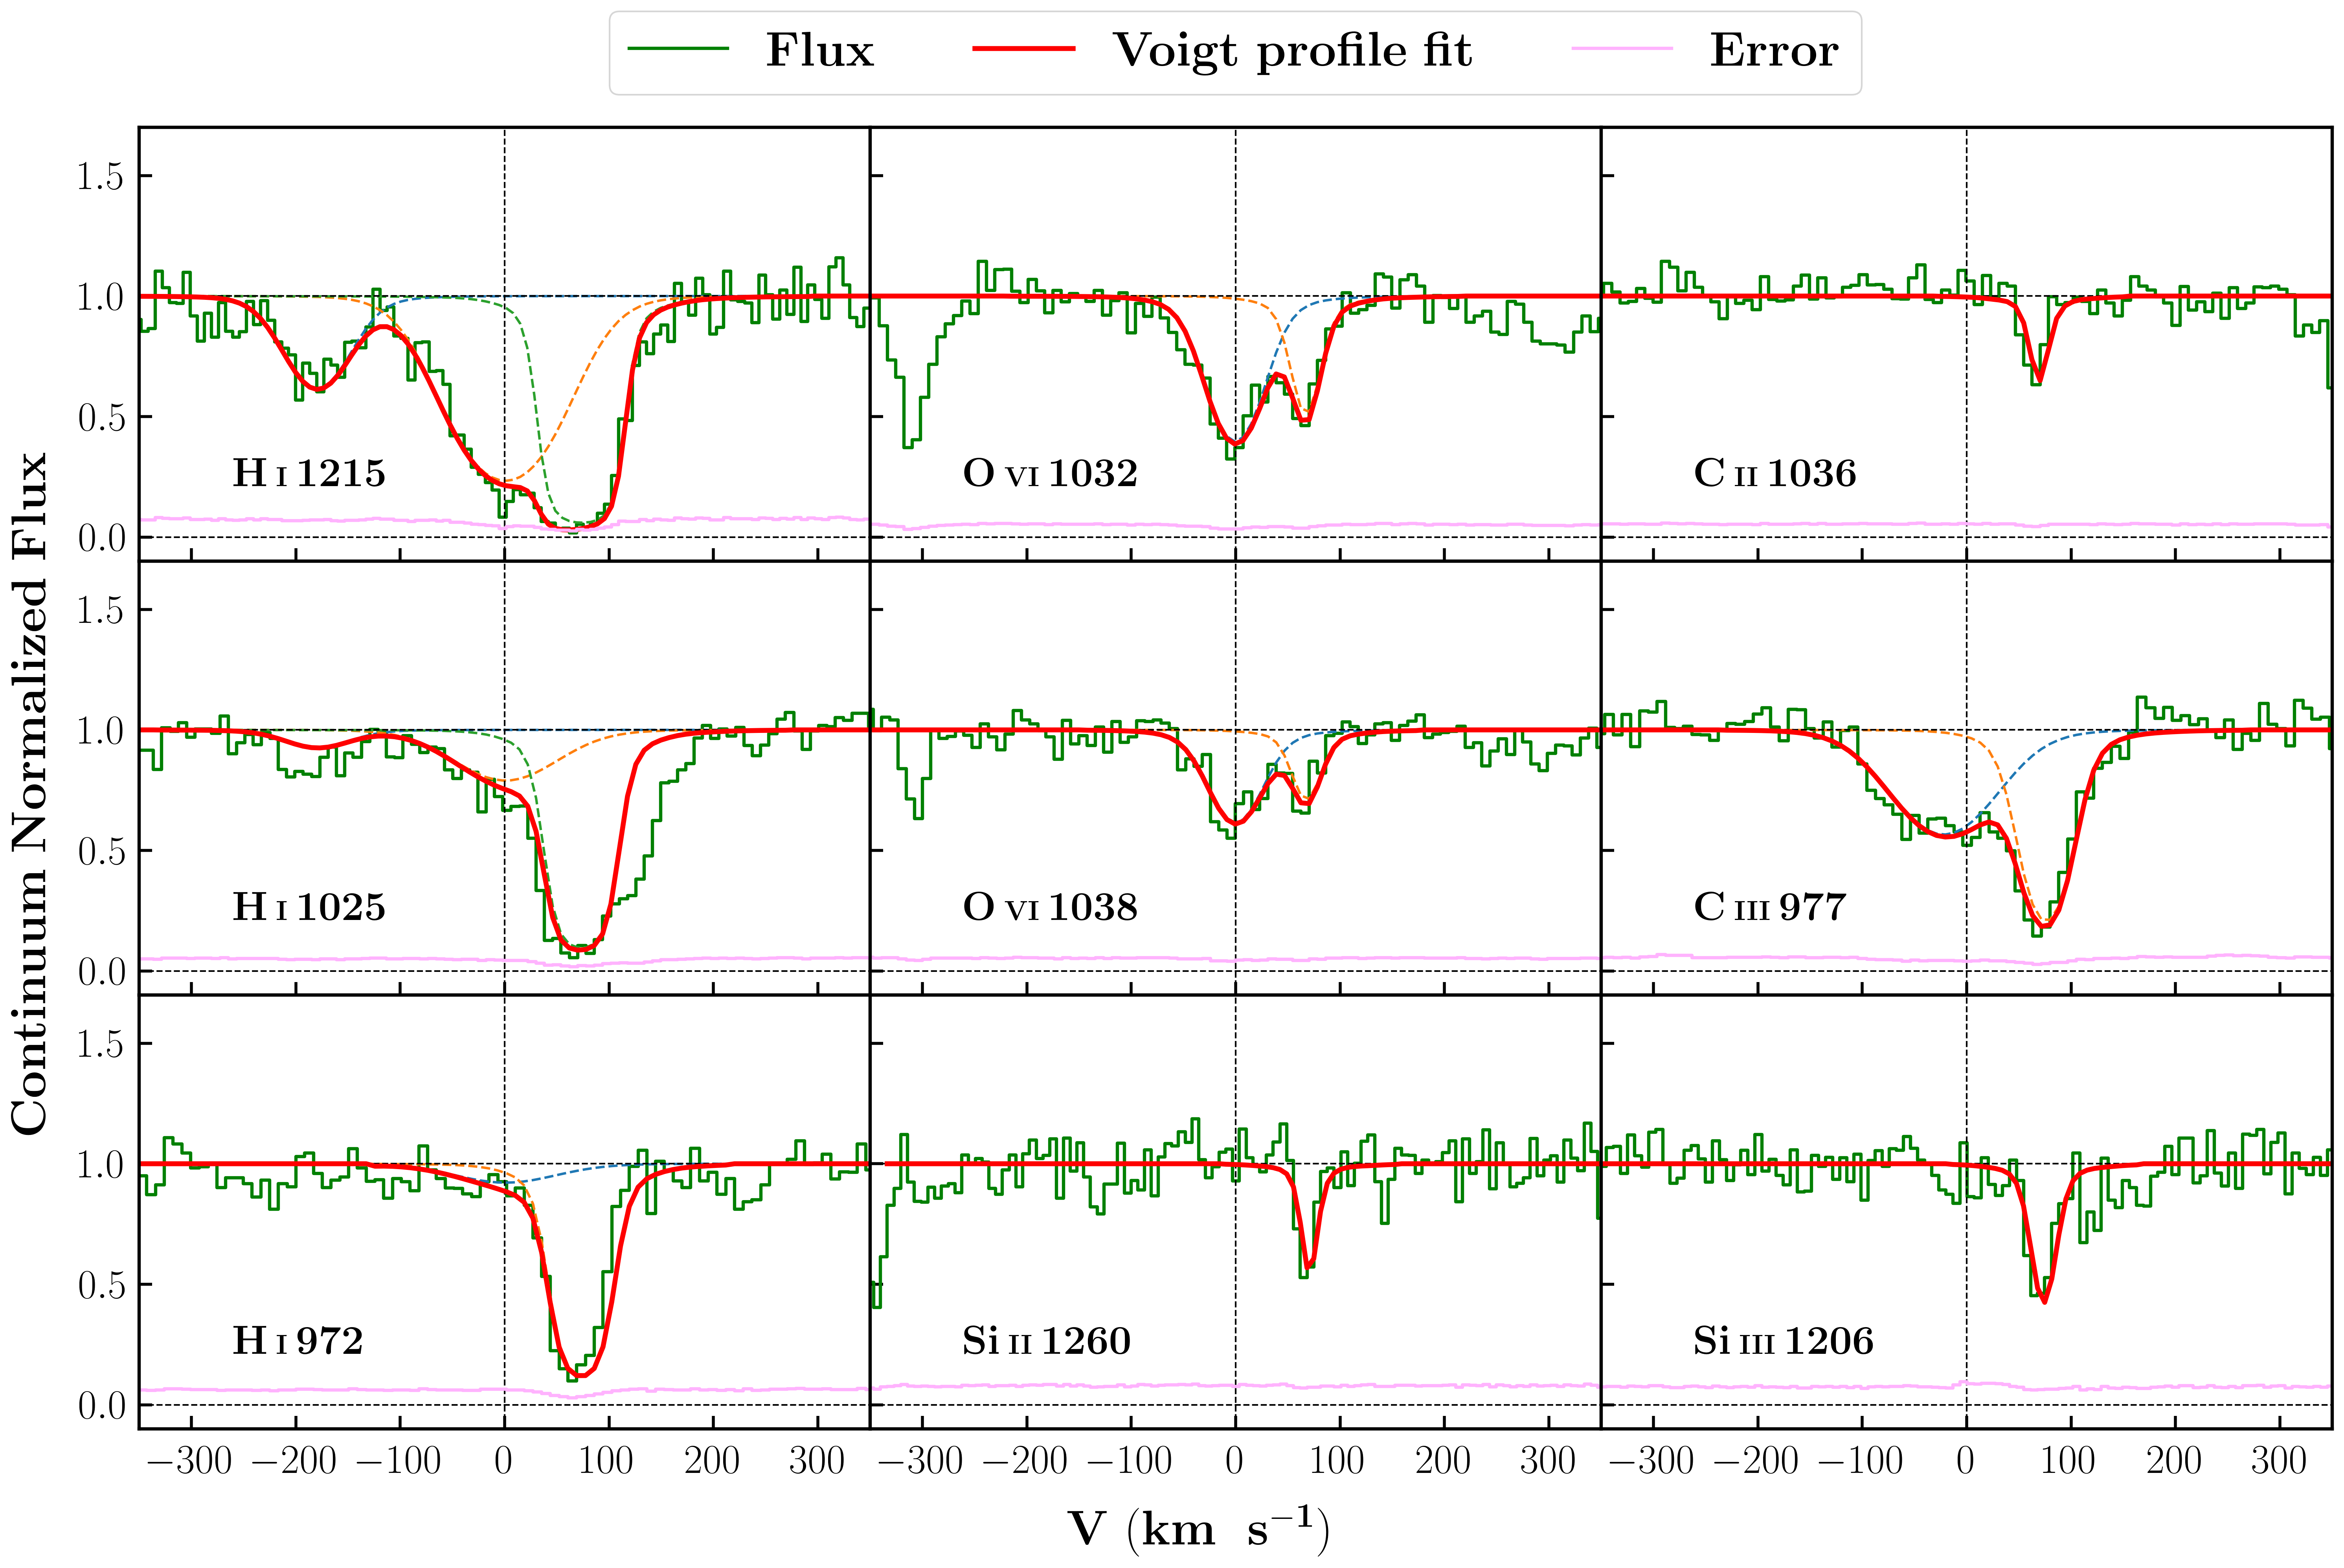
\includegraphics[width=10cm]{Figures/Mid-term/system_plot.jpg} % % \vspace*{-1mm} % % \caption{System plot of the absorber system. Velocity is taken to be zero at the redshift of \ion{O}{vi} line of component II, i.e. z = 0.347579} % % \end{figure}\markdownRendererInterblockSeparator
{}% \end{frame}\markdownRendererInterblockSeparator
{}\begin{frame}[plain,noframenumbering]{}\markdownRendererInterblockSeparator
{}\begin{figure}[!htbp] \centering \includegraphics[width=12cm]{Figures/Mid-term/PG0003+158-z=0.347579-sys-plot.png} \vspace*{-1mm} \caption{System plot of the absorber system. Velocity is taken zero at z = 0.347579} \end{figure}\markdownRendererInterblockSeparator
{}\end{frame}\markdownRendererInterblockSeparator
{}\begin{frame}{\huge{{\textbf{Voigt profile fitting}}}}\markdownRendererInterblockSeparator
{}\begin{columns} \begin{column}{0.4\textwidth} \vspace{-10mm} \begin{itemize} \item \ion{H}{i} : 3 components \item \ion{O}{vi} : 2 components \item \ion{C}{ii}, \ion{C}{iii}, \ion{Si}{ii}, \ion{Si}{iii} : 1 component \end{itemize} \end{column} \begin{column}{0.6\textwidth} \vspace{-3mm} \begin{figure}[!htbp] \centering 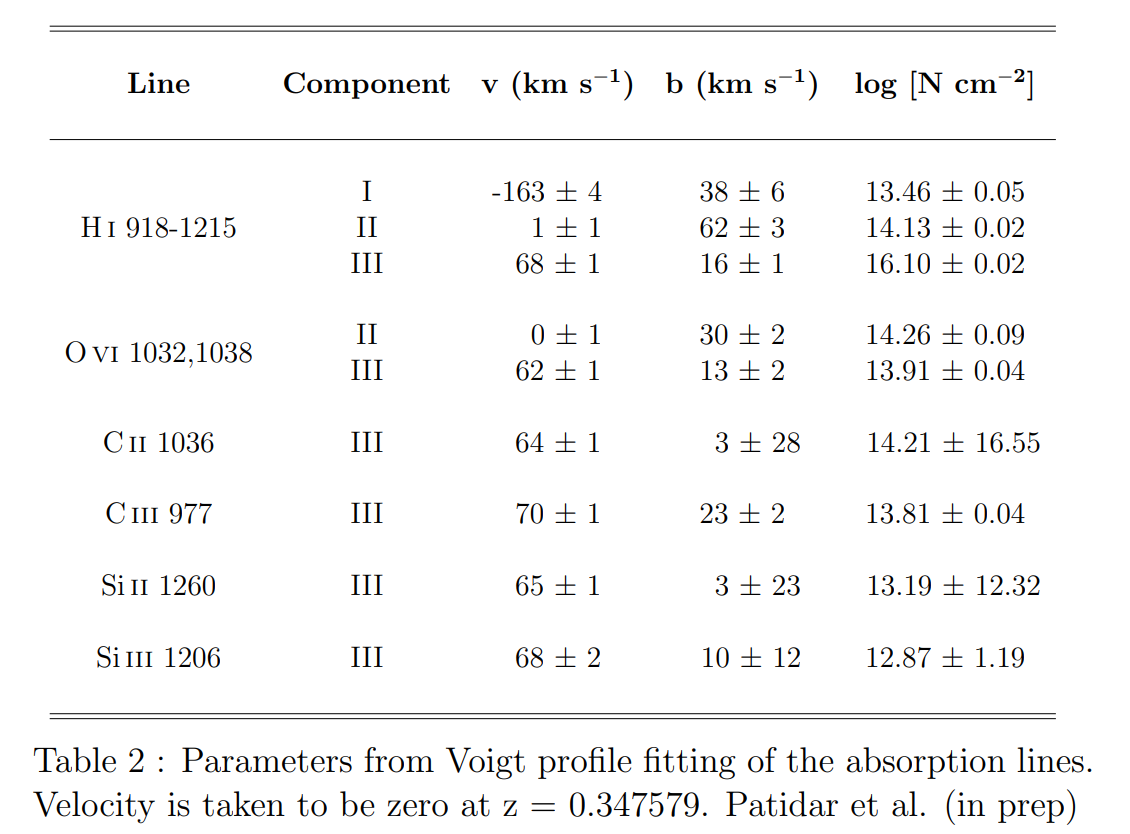
\includegraphics[width=8cm]{Figures/Mid-term/param.png} \end{figure} \end{column} \end{columns}\markdownRendererInterblockSeparator
{}\end{frame}\markdownRendererInterblockSeparator
{}\begin{frame}[noframenumbering]{\textbf{CLOUDY}}\markdownRendererInterblockSeparator
{}\begin{figure}[!htbp] \centering 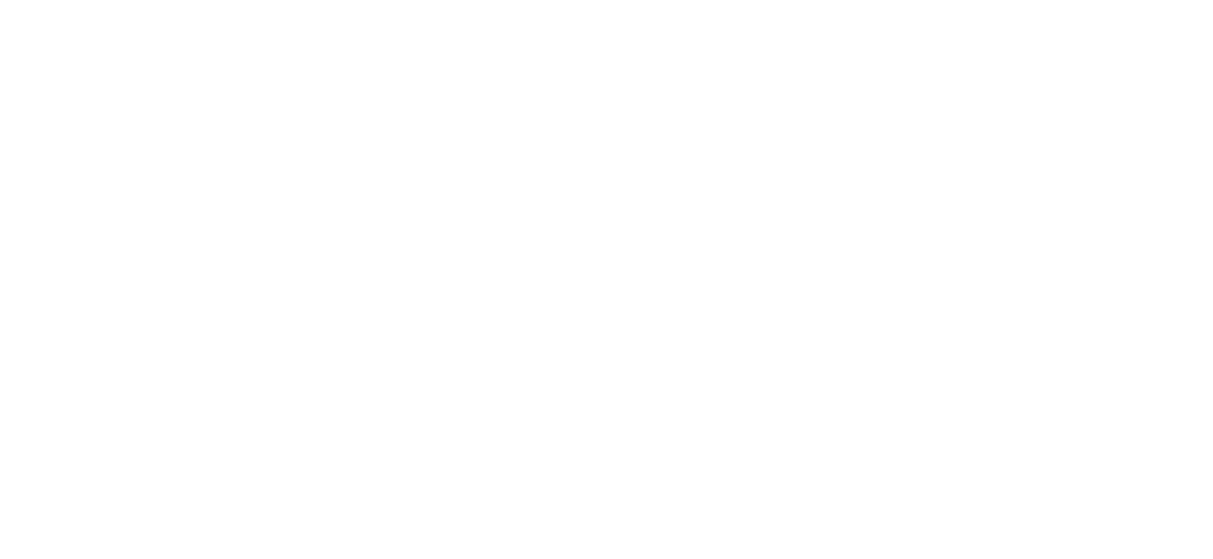
\includegraphics[width=12cm]{Figures/Mid-term/cloudy-transparent.png} \vspace*{-1mm} \caption{Schematic diagram of CLOUDY simulations.} \end{figure}\markdownRendererInterblockSeparator
{}\end{frame}\markdownRendererInterblockSeparator
{}\begin{frame}{\huge{{\textbf{Ionization Modelling}}}}\markdownRendererInterblockSeparator
{}\markdownRendererUlBegin
\markdownRendererUlItem Component I \ \ \ : -\markdownRendererUlItemEnd 
\markdownRendererUlItem Component II \ \ : Hybrid - Collisional + Photo-ionization\markdownRendererUlItemEnd 
\markdownRendererUlItem Component III \ : Photo-ionization (PI)\markdownRendererUlItemEnd 
\markdownRendererUlEnd \markdownRendererInterblockSeparator
{}\end{frame}\markdownRendererInterblockSeparator
{}\begin{frame}{\textbf{Component III : PI}}\markdownRendererInterblockSeparator
{}\uncover<1->{\begin{itemize} \uncover<2->{\item Grid of CLOUDY models : Density and Metallicity} \uncover<3->{\item log (${\text{n}}_{\text{H}} / \text{cm}^{-3}$) : -5 to 1 in steps of 0.02} \uncover<4->{\item log (Z/$Z\odot$) : -3 to 2 in steps of 0.05} \uncover<5->{\item Solution : Model that best matches the observed column densities} \end{itemize} }\markdownRendererInterblockSeparator
{}\begin{tikzpicture}[remember picture, overlay,use page relative coordinates]\markdownRendererInterblockSeparator
{}\uncover<2->{\node at (0.25,0.20) {Ref. : Acharya and Khaire (2021)}}\markdownRendererInterblockSeparator
{}\end{tikzpicture}\markdownRendererInterblockSeparator
{}\end{frame}\markdownRendererInterblockSeparator
{}\begin{frame}{}\markdownRendererInterblockSeparator
{}\begin{figure}[!htbp] \centering 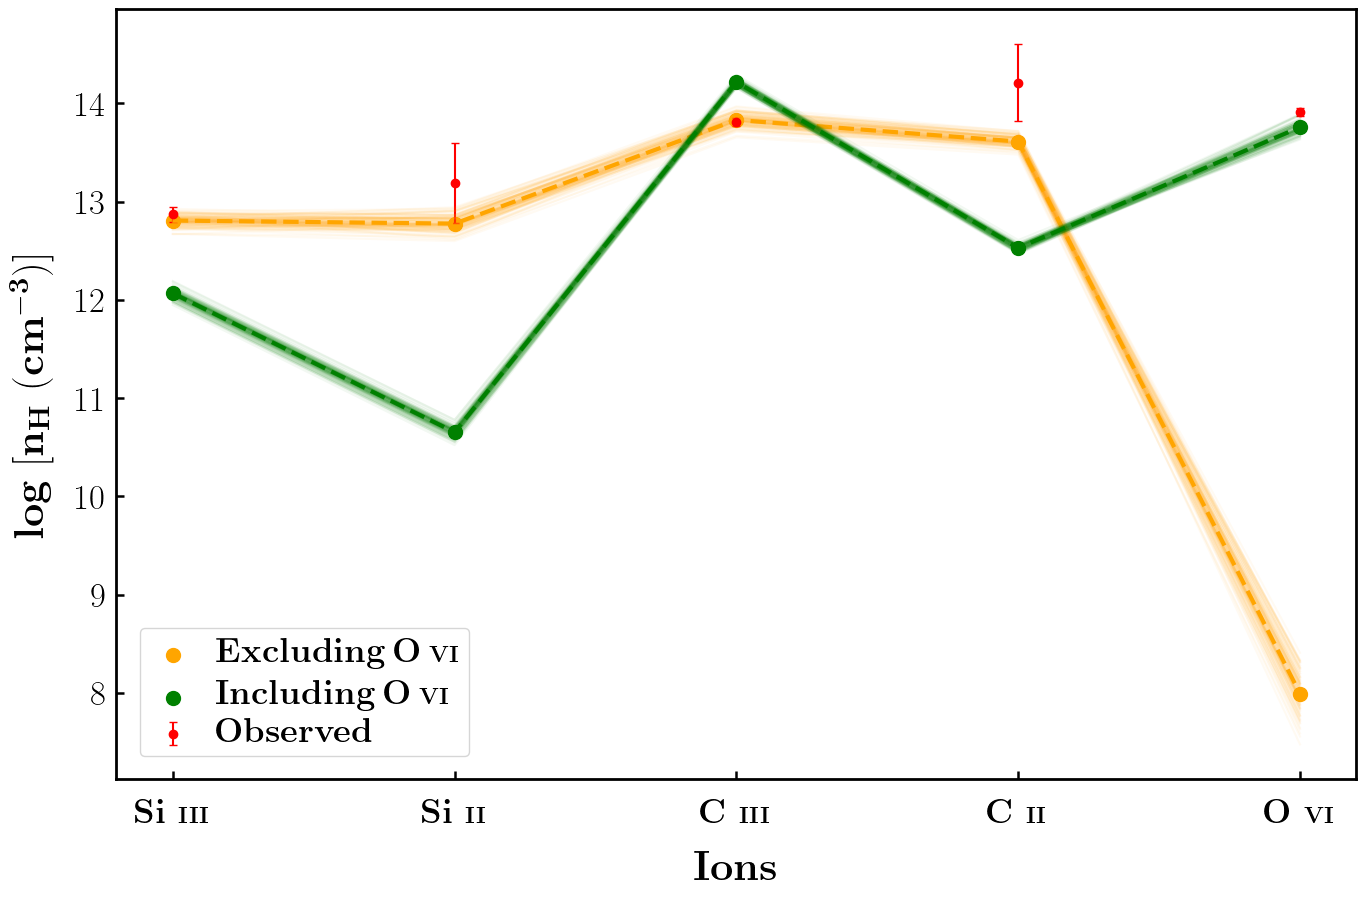
\includegraphics[width=10cm]{Figures/Mid-term/comp-III-PIE.png} \vspace*{-1mm} \caption{Modelled and observed column densities for the component III based on photoionization modelling} \end{figure}\markdownRendererInterblockSeparator
{}\end{frame}\markdownRendererInterblockSeparator
{}\begin{frame}{\textbf{Component II : Hybrid}}\markdownRendererInterblockSeparator
{}\vspace{-5mm}\markdownRendererInterblockSeparator
{}\uncover<1->{ \uncover<2->{\begin{center} {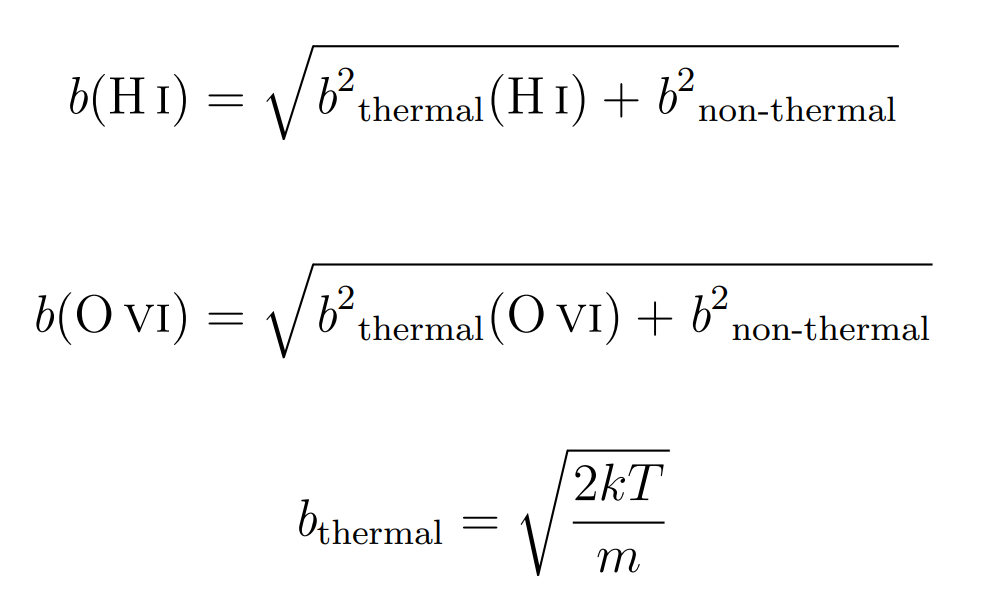
\includegraphics[width=5cm]{Figures/Mid-term/b3.png}} \end{center}} \begin{itemize} \uncover<3->{\item $T={10}^{{5.29}_{-0.08}^{+0.07}}$ K} \uncover<4->{\item Constant temperature CLOUDY models} \uncover<5->{\item \ion{O}{vi} and size as constraining factors} \end{itemize}}\markdownRendererInterblockSeparator
{}\end{frame}\markdownRendererInterblockSeparator
{}\begin{frame}{}\markdownRendererInterblockSeparator
{}\begin{figure}[!htbp] \centering 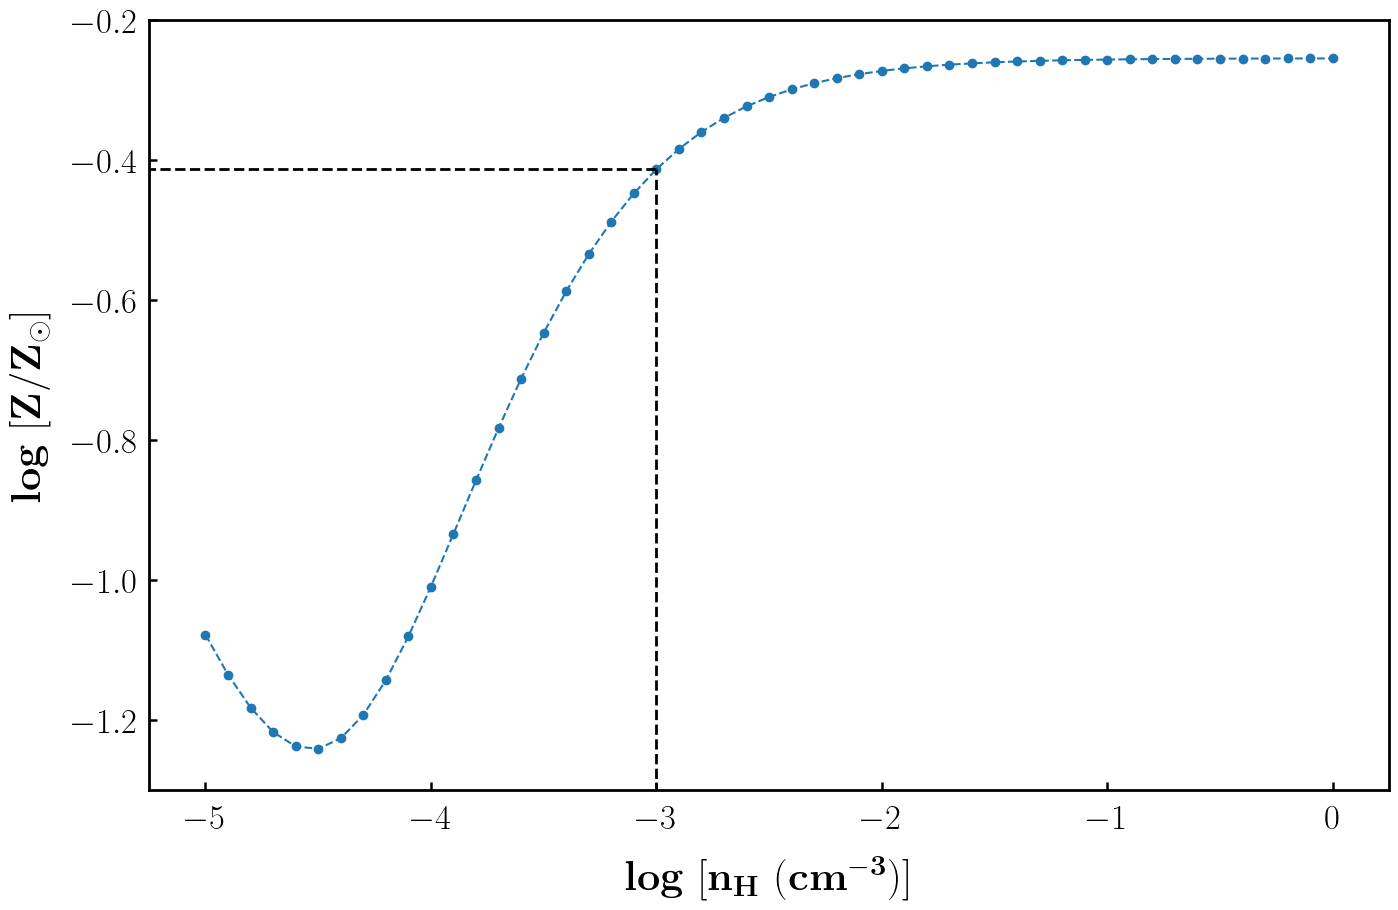
\includegraphics[width=10cm]{Figures/Mid-term/comp-II-CIE.png} \vspace*{-1mm} \caption{Hybrid model solution for component II.} \end{figure}\markdownRendererInterblockSeparator
{}\end{frame}\markdownRendererInterblockSeparator
{}\begin{frame}[noframenumbering]{}\markdownRendererInterblockSeparator
{}\begin{figure}[!htbp] \centering \includegraphics[width=14cm]{Figures/Mid-term/physical-params.png} \end{figure}\markdownRendererInterblockSeparator
{}\end{frame}\markdownRendererInterblockSeparator
{}\begin{frame}{\huge{{\textbf{Galaxy Environment}}}}\markdownRendererInterblockSeparator
{}\begin{columns} \begin{column}{0.4\textwidth} \vspace{-10mm} \uncover<1->{ \begin{itemize} \uncover<2->{\item Galaxies within 15\arcmin and 1000 km s$^{-1}$} \uncover<3->{\item SDSS : L $\gtrsim 2.77$ L$^*$} \uncover<4->{\item VIMOS \uncover<6->{: L $\gtrsim 0.07$ L$^*$}} \vspace{2mm} \uncover<7->{\item $r_{vir}=250\left(\frac{L}{L^{*}}\right)^{0.2}$ kpc} \end{itemize} \begin{tikzpicture}[remember picture, overlay,use page relative coordinates] \uncover<3->{\node at (0.18,0.15) {Ref. : Ilbert et al. (2005)}} \uncover<7->{\node at (0.24,0.10) {Prochaska et al. (2011)}} \end{tikzpicture} } \end{column} \begin{column}{0.6\textwidth} \vspace{-3mm} \uncover<5->{ \begin{figure}[!htbp] \centering 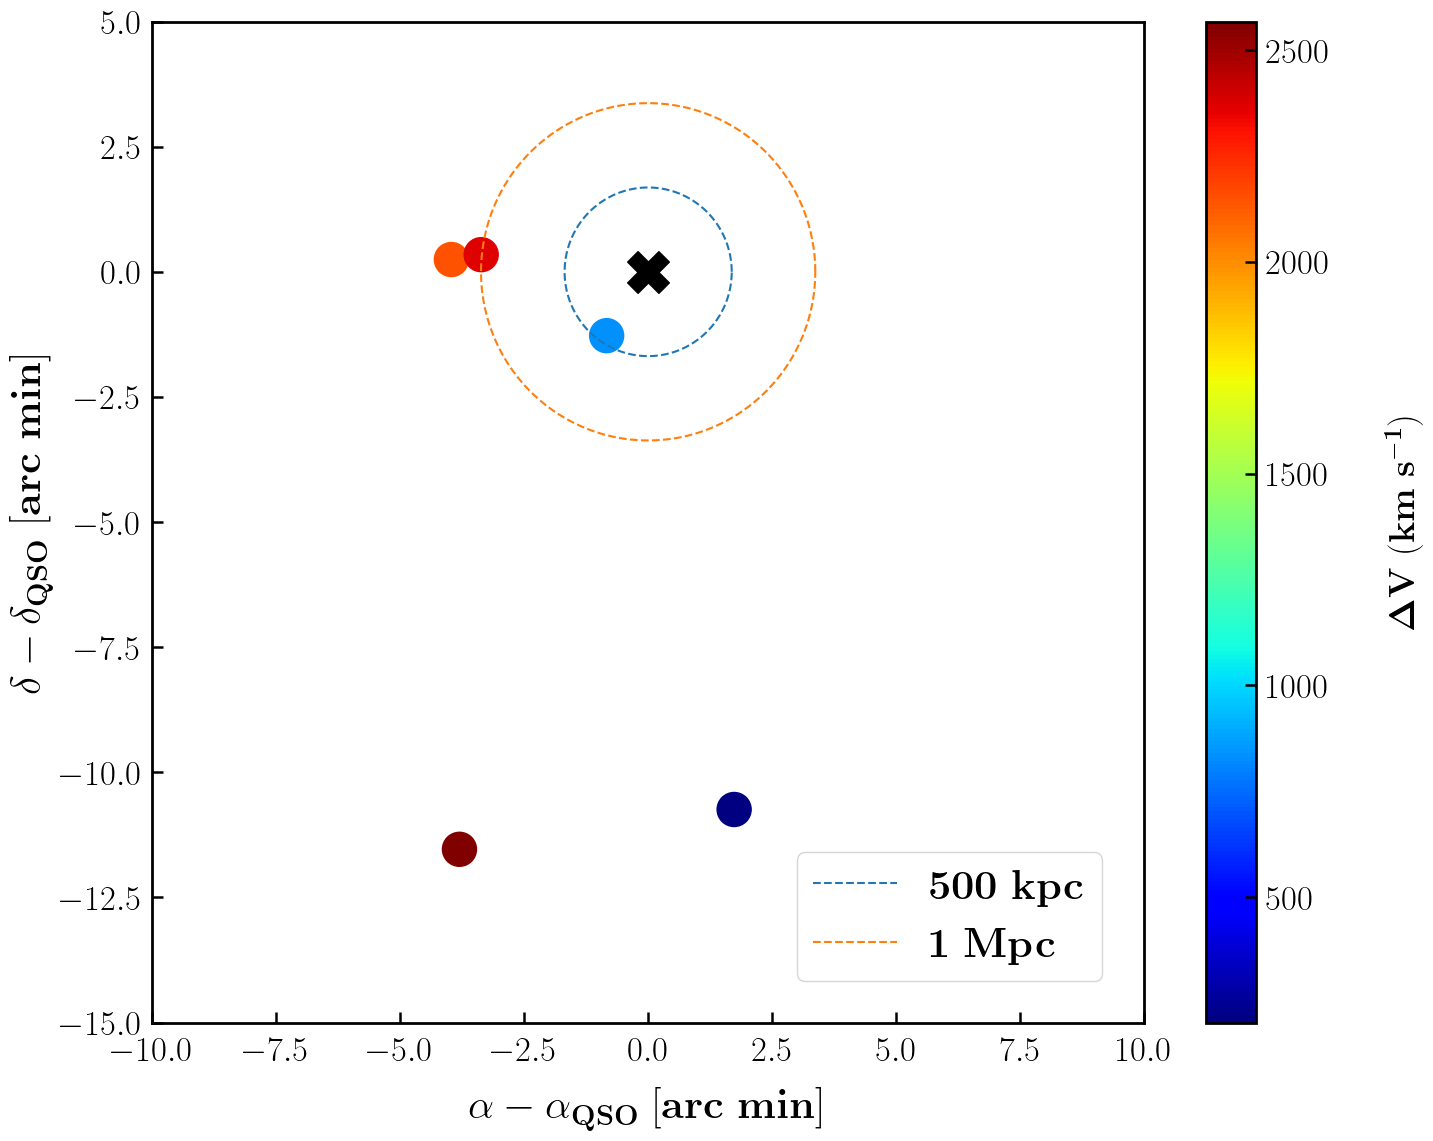
\includegraphics[width=7cm]{Figures/Mid-term/galaxy-environment.jpg} \vspace*{-1mm} \caption{Galaxies around the absorber color-coded with their velocity separation from the absorber. Velocity is 0 at z = 0.347579} \end{figure}} \end{column} \end{columns}\markdownRendererInterblockSeparator
{}\end{frame}\markdownRendererInterblockSeparator
{}\markdownRendererHeadingOne{Summary : Phase I}\markdownRendererInterblockSeparator
{}\vspace*{2.7cm}\markdownRendererInterblockSeparator
{}{\huge{\textbf{Summary : Phase I}}}\markdownRendererInterblockSeparator
{}\end{frame}\markdownRendererInterblockSeparator
{}\begin{frame}{\huge{{\textbf{Summary : Phase I}}}}\markdownRendererInterblockSeparator
{}\uncover<1-> { \begin{itemize} \uncover<2->{\item BLA candidate towards PG0003+158} \vspace{1mm} \begin{itemize} \uncover<3->{\item[-] Voigt profile fitting} \uncover<4->{\item[-] Ionisation modelling} \uncover<5->{\item[-] Galaxy environment} \end{itemize} \end{itemize} }\markdownRendererInterblockSeparator
{}\end{frame}\markdownRendererInterblockSeparator
{}\markdownRendererHeadingOne{The Survey}\markdownRendererInterblockSeparator
{}\vspace*{2.7cm}\markdownRendererInterblockSeparator
{}{\huge{\textbf{The Survey}}}\markdownRendererInterblockSeparator
{}\end{frame}\markdownRendererInterblockSeparator
{}\begin{frame}{\huge{\textbf{Hunt for BLAs}}}\markdownRendererInterblockSeparator
{}\uncover<1->{ \begin{itemize}\markdownRendererInterblockSeparator
{}\uncover<2->{\item Broad Ly$\alpha$ :}\markdownRendererInterblockSeparator
{}$$\uncover<3->{\MyBox{b \geq 45 \ \text{km s}^{-1}}} \uncover<4->{\hspace{8mm} \Rightarrow \ \ \ \text{568 systems}}$$\markdownRendererInterblockSeparator
{}\vspace{-3mm}\markdownRendererInterblockSeparator
{}\uncover<5->{\item Ionisation modelling :} \vspace{2mm} $$\uncover<6->{\MyBox{\text{metal ions} \geq 3}} \uncover<7->{\hspace{8mm} \Rightarrow \ \ \ \text{28 systems}}$$\markdownRendererInterblockSeparator
{}\begin{center} \vspace{2mm} \uncover<8->{\MyBox[red]{\textbf{28 BLA candidates}}} \end{center}\markdownRendererInterblockSeparator
{}\end{itemize} }\markdownRendererInterblockSeparator
{}\end{frame}\markdownRendererInterblockSeparator
{}\begin{frame}{} \begin{figure}[!htbp] \centering 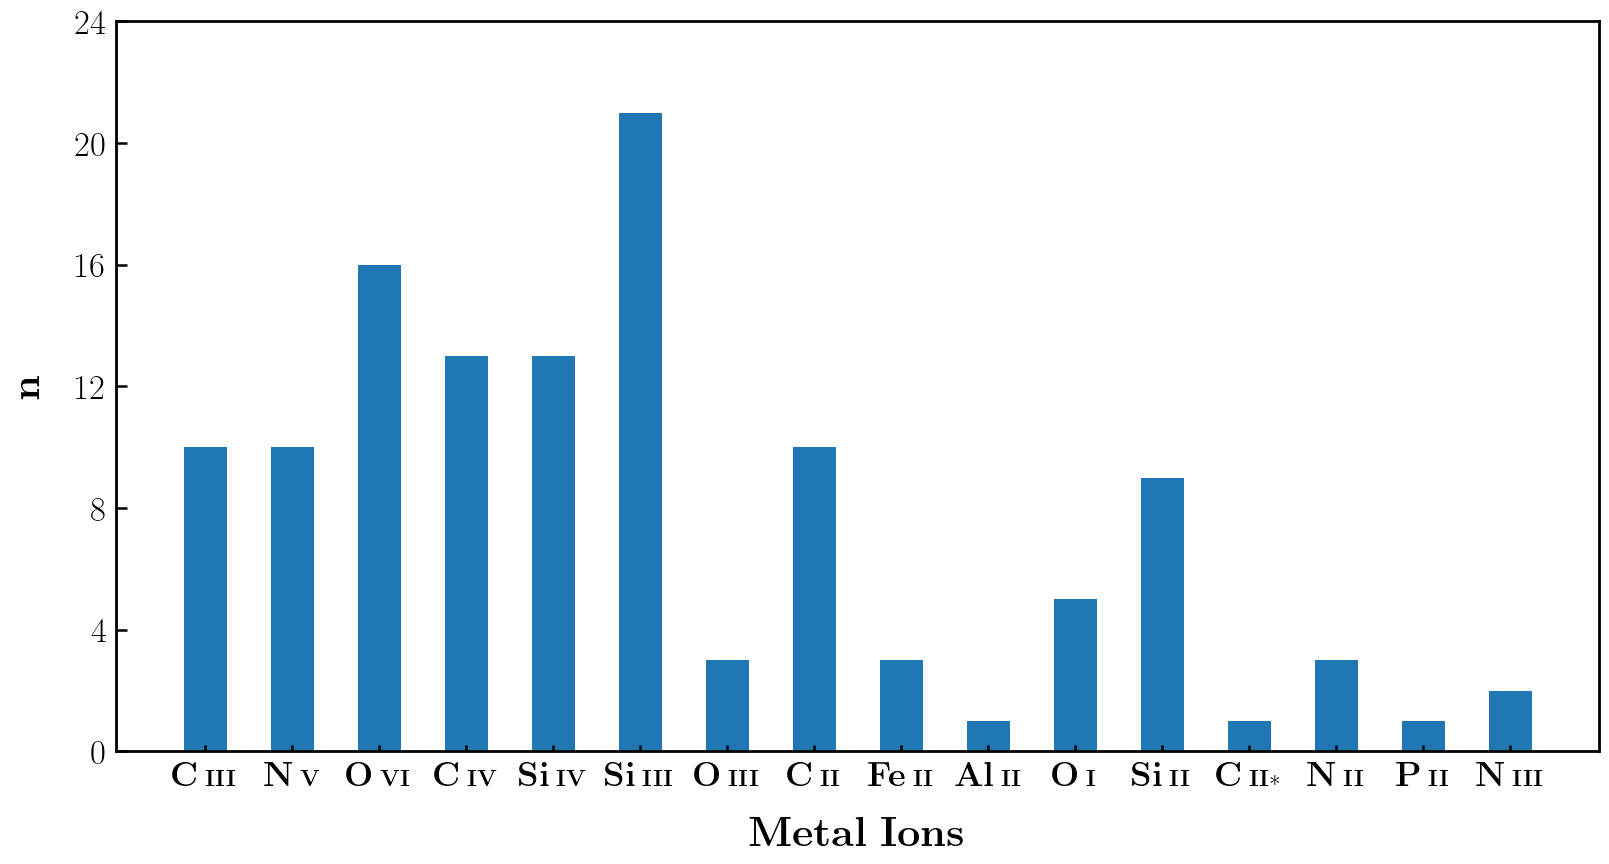
\includegraphics[width=12cm]{Figures/Mid-term/metal-ions.png} \vspace*{-1mm} \caption{No. of different metal ions in all the 28 candidate BLAs} \end{figure} \end{frame}\markdownRendererInterblockSeparator
{}\begin{frame}{\huge{\textbf{Survey so far}}}\markdownRendererInterblockSeparator
{}\uncover<1->{\begin{itemize} \uncover<2->{\item \ion{O}{vi} absorbers : 16} \uncover<3->{\item Voigt profile fitting \ \ \checkmark} \end{itemize}}\markdownRendererInterblockSeparator
{}\end{frame}\markdownRendererInterblockSeparator
{}\markdownRendererHeadingOne{Towards Thesis Phase II}\markdownRendererInterblockSeparator
{}\vspace*{2.7cm}\markdownRendererInterblockSeparator
{}{\huge{\textbf{Towards Thesis Phase II}}}\markdownRendererInterblockSeparator
{}\end{frame}\markdownRendererInterblockSeparator
{}\begin{frame}{\huge{\textbf{Towards Thesis Phase II}}}\markdownRendererInterblockSeparator
{}\markdownRendererUlBegin
\markdownRendererUlItem Ionisation modelling of \ion{O}{vi} absorbers\markdownRendererUlItemEnd 
\markdownRendererUlItem Galaxy environments of these absorbers\markdownRendererUlItemEnd 
\markdownRendererUlItem Studying remaining 12 absorbers\markdownRendererUlItemEnd 
\markdownRendererUlItem Contribution of BLAs to $\Omega_b$\markdownRendererUlItemEnd 
\markdownRendererUlEnd \markdownRendererInterblockSeparator
{}\end{frame}\markdownRendererInterblockSeparator
{}% \uncover<1->{\begin{itemize} % \uncover<2->{\item } % \uncover<3->{\item } % \uncover<4->{\item } % \uncover<5->{\item } % \end{itemize}}\markdownRendererInterblockSeparator
{}% \begin{columns} % \begin{column}{0.6\textwidth} % \begin{itemize} % \uncover<1->{\item Baryon surveys showed deficiency in baryon count} % \uncover<2->{\item } % \uncover<3->{\item } % \uncover<4->{\item } % \uncover<5->{\item } % \uncover<6->{\item } % \end{itemize} % \end{column} % \begin{column}{0.4\textwidth} % \begin{figure}[!htbp] % \centering % \includegraphics[width=5cm]{Placeholder.png} % \vspace*{-1mm} % \caption{} % \label{} % \end{figure} % \end{column} % \end{columns}\markdownRendererInterblockSeparator
{}%% ----------- References ----------\markdownRendererInterblockSeparator
{}\begin{frame}<presentation:0>[noframenumbering]\markdownRendererInterblockSeparator
{}{\cite{Fukugita-1998} \cite{Shull} \cite{cen-ostriker-1999} \cite{tepper-2013} \cite{savage-2014} \cite{danforth-2016} \cite{acharya_khaire}}\markdownRendererInterblockSeparator
{}\end{frame}\markdownRendererInterblockSeparator
{}% \end{frame}\markdownRendererInterblockSeparator
{}\begin{frame} \renewcommand{\bibfont}{\footnotesize} \frametitle{\huge{\textbf{References}}}\markdownRendererInterblockSeparator
{}\bibliographystyle{mnras} \bibliography{References}\markdownRendererInterblockSeparator
{}\end{frame}\markdownRendererInterblockSeparator
{}\begin{frame}{} \centering \Huge \textbf{\emph{Seek understanding, not $\chi^2=1$}} \end{frame}\relax